This project is a proof-of-concept of a swedish question answering system, similiar to IBM Watson.
The goal is to create a system that is able to answer simple questions with one word long answers.
To do this we use the swedish wikipedia as our data source and annotated questions from the swedish 
board game Kvitt eller dubbelt as our training questions and categories.

A system overview is shown in figure \ref{fig:overview}. 

\begin{figure*}
\centering
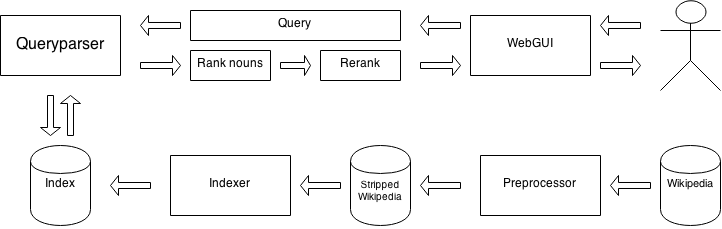
\includegraphics[width=1\textwidth]{figures/Question-answering-system.png}
\caption{Overview}
\label{fig:overview}
\end{figure*}
